\documentclass[aspectratio=169,11pt]{beamer}
\usetheme{metropolis}
\usepackage{tikz}
\usetikzlibrary{arrows.meta,positioning,calc}
\usepackage{booktabs}
\usepackage{xcolor}
\usepackage{amsmath}
\usepackage{hyperref}

% === Color palette ===
\definecolor{report}{HTML}{3498DB}
\definecolor{state}{HTML}{9B59B6}
\definecolor{bias}{HTML}{E67E22}
\definecolor{neutral}{HTML}{95A5A6}
\definecolor{pass}{HTML}{27AE60}
\definecolor{fail}{HTML}{E74C3C}
\tikzset{
  box/.style={draw=#1,thick,rounded corners,fill=#1!10,minimum width=3.2cm,minimum height=0.9cm,font=\small,align=center},
  boxL/.style={draw=#1,thick,rounded corners,fill=#1!10,minimum width=5.2cm,minimum height=1.2cm,font=\small,align=center},
  boxS/.style={draw=#1,thick,rounded corners,fill=#1!10,minimum width=2.8cm,minimum height=0.9cm,font=\footnotesize,align=center},
}
\hypersetup{colorlinks=true,linkcolor=.,urlcolor=report}

\title{Reports as Measurements}
\subtitle{Matthias Michel's consciousness science, applied to LLM introspection}
\author{Measuring AI Introspection}
\date{}
\institute{}

\newcommand{\partslide}[2]{%
\begin{frame}[plain,label=#1]
\vfill
\begin{center}
  \setlength{\fboxrule}{2.5pt}%
  \fcolorbox{black}{white}{\parbox{0.65\textwidth}{\centering\vspace{0.8em}
    {\Large\bfseries #2}
  \vspace{0.8em}}}
\end{center}
\vfill
\end{frame}}

\begin{document}

\maketitle

%% --- Overview ---
\begin{frame}{Overview}\footnotesize
\begin{columns}[T]
\begin{column}{0.48\textwidth}
\hyperlink{part1}{\textbf{Part 1: The problem}}\\[0.15em]
{\scriptsize%
\quad\hyperlink{flash}{1.~Did you see it?}\\%
\quad\hyperlink{twosteps}{2.~Two steps from answer to claim}\\%
\quad\hyperlink{llm}{3.~The same problem in an LLM}%
}\vspace{0.3em}

\hyperlink{part2}{\textbf{Part 2: The right quantity?}}\\[0.15em]
{\scriptsize%
\quad\hyperlink{thermo}{4.~A bad thermometer vs.\ the wrong instrument}\\%
\quad\hyperlink{circle}{5.~The circle}\\%
\quad\hyperlink{commoncause}{6.~Agreement can have a common cause}%
}\vspace{0.3em}

\hyperlink{part3}{\textbf{Part 3: Calibration}}\\[0.15em]
{\scriptsize%
\quad\hyperlink{concordance}{7.~Check it against a different instrument}\\%
\quad\hyperlink{modelcal}{8.~Model how the instrument could go wrong}\\%
\quad\hyperlink{averaging}{9.~What averaging fixes, and what it cannot}%
}
\end{column}
\begin{column}{0.48\textwidth}
\hyperlink{part4}{\textbf{Part 4: Saying yes}}\\[0.15em]
{\scriptsize%
\quad\hyperlink{scale}{10.~The criterion problem}\\%
\quad\hyperlink{sdt}{11.~Signal detection in one picture}\\%
\quad\hyperlink{yesbias}{12.~Injection makes the model say yes}\\%
\quad\hyperlink{metad}{13.~How much of what it knows reaches the report?}\\%
\quad\hyperlink{content}{14.~Credit for noticing something}%
}\vspace{0.3em}

\hyperlink{part5}{\textbf{Part 5: Drift and limits}}\\[0.15em]
{\scriptsize%
\quad\hyperlink{drift}{15.~Validity drift}\\%
\quad\hyperlink{limits}{16.~Where the analogy stops}\\%
\quad\hyperlink{summary}{17.~Summary}\\%
\quad\hyperlink{reading}{18.~Reading}%
}
\end{column}
\end{columns}
\end{frame}

%% ============================================================
\partslide{part1}{Part 1\\[0.5em]{\large\mdseries The problem}}
%% ============================================================

\begin{frame}[label=flash]{Did you see it?}
A consciousness experiment, in its simplest form:

\vspace{0.5em}
\begin{enumerate}\setlength\itemsep{6pt}
  \item {\small A word is flashed on a screen for 30 milliseconds, then covered by a pattern (a \emph{mask}).}
  \item {\small The subject is asked: \emph{did you see a word?}}
  \item {\small Repeat a few hundred times, with and without a word.}
\end{enumerate}

\vspace{0.5em}
The researcher wants to know whether the subject was \textbf{conscious} of the word. The only thing the researcher gets is the \textbf{answer}.

\vspace{0.5em}
{\small So every conclusion about consciousness passes through a decision about what an answer means.
\href{https://philpapers.org/archive/MICTMO-15.pdf}{Matthias Michel}'s work has studied this decision using the tools of measurement theory, drawing on Eran Tal and Hasok Chang.}
\end{frame}

\begin{frame}[label=twosteps]{Two steps from answer to claim}
Michel splits the path from experience to conclusion into two steps:

\vspace{0.6em}
\begin{center}
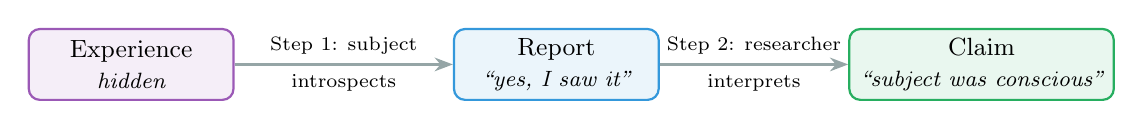
\begin{tikzpicture}
  \node[box=state,minimum width=2.6cm] (exp) at (0,0) {Experience\\{\footnotesize\itshape hidden}};
  \node[box=report,minimum width=2.6cm] (rep) at (5.4,0) {Report\\{\footnotesize\itshape ``yes, I saw it''}};
  \node[box=pass,minimum width=2.6cm] (claim) at (10.8,0) {Claim\\{\footnotesize\itshape ``subject was conscious''}};
  \draw[-{Stealth},thick,neutral] (exp) -- node[above,font=\scriptsize,text=black]{Step 1: subject} node[below,font=\scriptsize,text=black]{introspects} (rep);
  \draw[-{Stealth},thick,neutral] (rep) -- node[above,font=\scriptsize,text=black]{Step 2: researcher} node[below,font=\scriptsize,text=black]{interprets} (claim);
\end{tikzpicture}
\end{center}

\vspace{0.6em}
In measurement language, the report is an \textbf{\textcolor{report}{indication}}: what the instrument shows, like the height of mercury in a thermometer.
The claim is the \textbf{measurement outcome}, and getting from one to the other needs a model of the instrument.

\vspace{0.4em}
{\small Most worries about self-report are about Step 1 (is the subject accurate?). Michel's main worry is Step 2: should the answer be read as a reading of consciousness at all?}
\end{frame}

\begin{frame}[label=llm]{The same problem in an LLM}
\href{https://arxiv.org/abs/2601.01828}{Lindsey (2025)} runs the LLM version of the flash experiment:

\vspace{0.5em}
\begin{enumerate}\setlength\itemsep{5pt}
  \item {\small Take the model's internal activation pattern for a word, such as \emph{bread}.}
  \item {\small Add it to the model's activations while it answers a question (\emph{concept injection}).}
  \item {\small Ask: \emph{Do you detect an injected thought? If so, what is it about?}}
\end{enumerate}

\vspace{0.5em}
\begin{columns}[T]
\begin{column}{0.48\textwidth}
{\small\textbf{Consciousness experiment}}\\
{\footnotesize flashed word $\to$ experience $\to$ ``I saw it''}
\end{column}
\begin{column}{0.48\textwidth}
{\small\textbf{Introspection experiment}}\\
{\footnotesize injected vector $\to$ internal state $\to$ ``I detect a thought about bread''}
\end{column}
\end{columns}

\vspace{0.6em}
{\small Michel writes about people and animals, not language models. The structure carries over anyway: the researcher changes something hidden, gets an answer, and has to decide what the answer measures.}
\end{frame}

%% ============================================================
\partslide{part2}{Part 2\\[0.5em]{\large\mdseries Is it measuring the right thing?}}
%% ============================================================

\begin{frame}[label=thermo]{A bad thermometer vs.\ the wrong instrument}
Michel's example (\href{https://philarchive.org/archive/MICCIC-3}{2023}, p.~16):

\vspace{0.5em}
\begin{columns}[T]
\begin{column}{0.48\textwidth}
\begin{center}
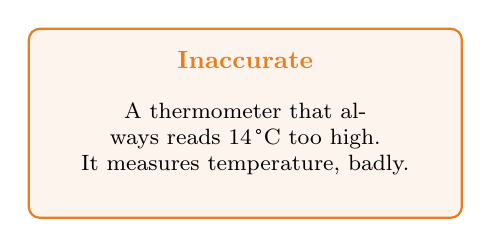
\begin{tikzpicture}
  \draw[bias,thick,rounded corners,fill=bias!8] (0,0) rectangle (5.5,2.4);
  \node[font=\small\bfseries,bias] at (2.75,2.0) {Inaccurate};
  \node[font=\footnotesize,align=center,text width=5cm] at (2.75,1.0) {A thermometer that always reads 14\,°C too high.\\It measures temperature, badly.};
\end{tikzpicture}
\end{center}
\end{column}
\begin{column}{0.48\textwidth}
\begin{center}
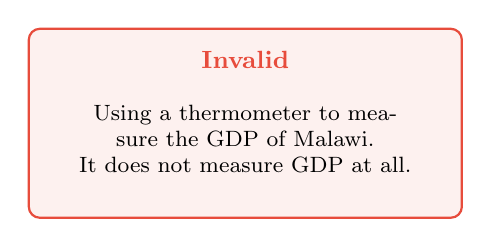
\begin{tikzpicture}
  \draw[fail,thick,rounded corners,fill=fail!8] (0,0) rectangle (5.5,2.4);
  \node[font=\small\bfseries,fail] at (2.75,2.0) {Invalid};
  \node[font=\footnotesize,align=center,text width=5cm] at (2.75,1.0) {Using a thermometer to measure the GDP of Malawi.\\It does not measure GDP at all.};
\end{tikzpicture}
\end{center}
\end{column}
\end{columns}

\vspace{0.6em}
\textbf{Accuracy} asks how close the reading is. \textbf{Validity} asks whether the reading is about the right quantity.

\vspace{0.4em}
{\small For introspection: a model that reports injected thoughts 20\% of the time might be an inaccurate introspector, or its reports might track something else, such as how strange its own output looks.}
\end{frame}

\begin{frame}[label=circle]{The circle}
To show that reports measure consciousness, you need a theory of consciousness. To test the theory, you need a measure.

\vspace{0.4em}
\begin{center}
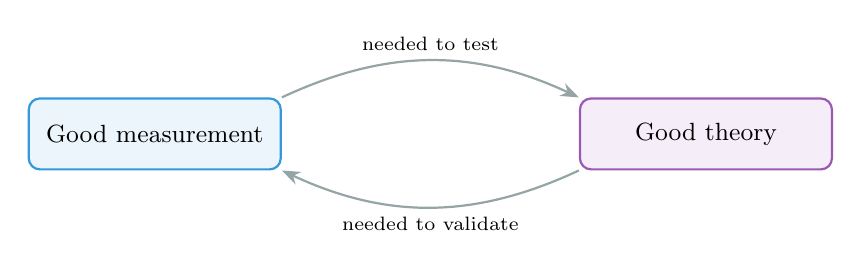
\begin{tikzpicture}
  \node[box=report] (m) at (0,0) {Good measurement};
  \node[box=state] (t) at (7,0) {Good theory};
  \draw[-{Stealth},thick,neutral] (m.north east) to[bend left=25] node[above,font=\scriptsize,text=black]{needed to test} (t.north west);
  \draw[-{Stealth},thick,neutral] (t.south west) to[bend left=25] node[below,font=\scriptsize,text=black]{needed to validate} (m.south east);
\end{tikzpicture}
\end{center}

\vspace{0.3em}
Michel calls this the \textbf{coordination problem}. Thermometry had the same circle, and Hasok Chang (\emph{Inventing Temperature}, 2004) describes how it got out by iteration.

\vspace{0.3em}
{\small For LLMs: checking a report against the injected vector assumes the vector \emph{is} the state being introspected.}
\end{frame}

\begin{frame}[label=commoncause]{Agreement can have a common cause}
A natural check: people who say ``I saw it'' also identify the word better. Doesn't that show the reports are valid?

\vspace{0.5em}
\begin{center}
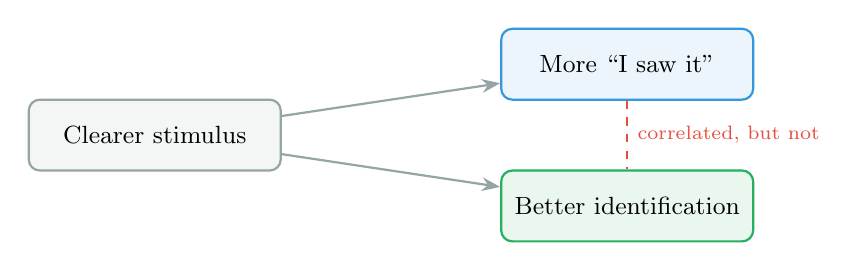
\begin{tikzpicture}
  \node[box=neutral] (c) at (0,0) {Clearer stimulus};
  \node[box=report] (r) at (6,0.9) {More ``I saw it''};
  \node[box=pass] (p) at (6,-0.9) {Better identification};
  \draw[-{Stealth},thick,neutral] (c) -- (r);
  \draw[-{Stealth},thick,neutral] (c) -- (p);
  \draw[dashed,fail,thick] (r) -- node[right,font=\scriptsize,text=fail]{correlated, but not} (p);
\end{tikzpicture}
\end{center}

\vspace{0.2em}
Michel's point (\href{https://philpapers.org/archive/MICTMO-15.pdf}{2019}): clearer stimuli improve both, so the correlation does not need consciousness to explain it.

\vspace{0.3em}
{\small For LLMs: if a stronger injection raises both the report rate and a probe's accuracy, the two agree because of injection strength alone.}
\end{frame}

%% ============================================================
\partslide{part3}{Part 3\\[0.5em]{\large\mdseries Calibrating without ground truth}}
%% ============================================================

\begin{frame}[label=concordance]{Check it against a different instrument}
In \href{https://philpapers.org/archive/MICCIC-2.pdf}{Calibration in Consciousness Science} (2021), Michel describes two ways to calibrate when there is no ground truth. The first is \textbf{concordance-calibration}:

\vspace{0.5em}
\begin{center}
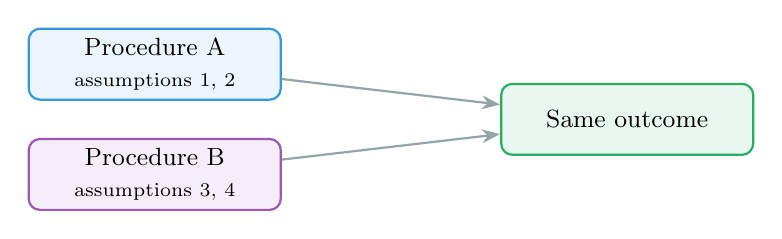
\begin{tikzpicture}
  \node[box=report] (a) at (0,0) {Procedure A\\{\scriptsize assumptions 1, 2}};
  \node[box=state] (b) at (0,-1.4) {Procedure B\\{\scriptsize assumptions 3, 4}};
  \node[box=pass] (o) at (6,-0.7) {Same outcome};
  \draw[-{Stealth},thick,neutral] (a) -- (o);
  \draw[-{Stealth},thick,neutral] (b) -- (o);
\end{tikzpicture}
\end{center}

\vspace{0.4em}
If two procedures that rest on \textbf{different assumptions} agree, a shared error becomes less likely.

\vspace{0.3em}
{\small For LLMs: does the report agree with a probe, an ablation, or another model watching the same trials? Only if they do not share a weak assumption.}
\end{frame}

\begin{frame}[label=modelcal]{Model how the instrument could go wrong}
The second is \textbf{model-calibration}: build a model of how the procedure works, then predict what it would output if a particular error were present.

\vspace{0.5em}
\begin{columns}[T]
\begin{column}{0.48\textwidth}
{\small\textbf{Michel's case}}\\[0.2em]
{\footnotesize Subjects bet money on whether they saw a stimulus. Fleming and Dolan (2010) modeled an ideal bettor and found the bets were distorted by \textbf{loss aversion}, not only by what subjects saw.}
\end{column}
\begin{column}{0.48\textwidth}
{\small\textbf{LLM version}}\\[0.2em]
{\footnotesize Suppose the prompt makes the model inclined to answer yes. Model that: predict how often a yes-biased model with no access to the injection would say ``detected'', and compare with what it does.}
\end{column}
\end{columns}

\vspace{0.8em}
{\small Michel's rule: you do not have to model everything that could affect a report, only the factors that would cause \textbf{systematic} errors.}
\end{frame}

\begin{frame}[label=averaging]{What averaging fixes, and what it cannot}
Random errors shrink when you average over many trials and many subjects. Systematic errors do not.

\vspace{0.6em}
\begin{center}
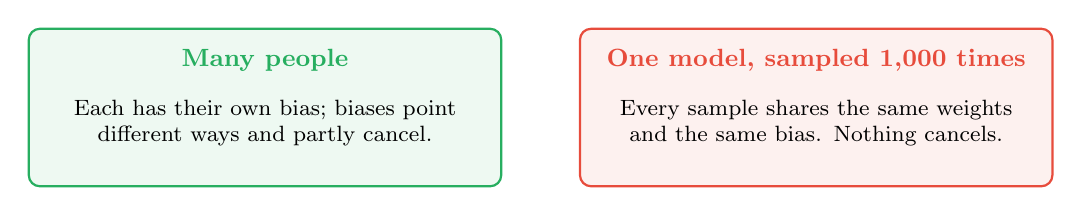
\begin{tikzpicture}
  \draw[pass,thick,rounded corners,fill=pass!8] (0,0) rectangle (6,2);
  \node[font=\small\bfseries,pass] at (3,1.6) {Many people};
  \node[font=\footnotesize,align=center,text width=5.5cm] at (3,0.8) {Each has their own bias; biases point different ways and partly cancel.};
  \draw[fail,thick,rounded corners,fill=fail!8] (7,0) rectangle (13,2);
  \node[font=\small\bfseries,fail] at (10,1.6) {One model, sampled 1{,}000 times};
  \node[font=\footnotesize,align=center,text width=5.5cm] at (10,0.8) {Every sample shares the same weights and the same bias. Nothing cancels.};
\end{tikzpicture}
\end{center}

\vspace{0.5em}
Michel's argument assumes ``that biases are more or less randomly distributed across subjects'' (2021, p.~17).
A single LLM is \textbf{one subject}, however many times you sample it.
\end{frame}

%% ============================================================
\partslide{part4}{Part 4\\[0.5em]{\large\mdseries The tendency to say yes}}
%% ============================================================

\begin{frame}[label=scale]{The criterion problem}
A subject says ``I didn't see it.'' Two very different explanations:

\vspace{0.5em}
\begin{enumerate}\setlength\itemsep{5pt}
  \item {\small They had no experience of the word.}
  \item {\small They had a faint experience, and only say ``yes'' when they are very sure.}
\end{enumerate}

\vspace{0.5em}
The second is a strict \textbf{\textcolor{bias}{criterion}}. Michel's analogy (\href{https://philpapers.org/archive/MICTOA-2.pdf}{2023}, p.~137): a bathroom scale that always reads slightly low. Trust it blindly and you might conclude that some light objects weigh nothing. Correct for the bias and they don't.

\vspace{0.5em}
{\small For LLMs: a model that rarely says ``I detect an injected thought'' may detect nothing, or may be trained to be cautious about claiming inner experiences.}
\end{frame}

\begin{frame}[label=sdt]{Signal detection in one picture}
\begin{columns}[T]
\begin{column}{0.55\textwidth}
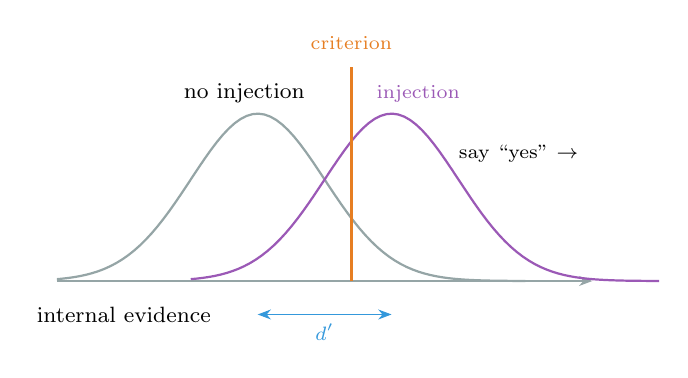
\begin{tikzpicture}[scale=0.85]
  \draw[-{Stealth},neutral] (-3,0) -- (5,0);
  \node[font=\footnotesize,text=black] at (-2,-0.5) {internal evidence};
  \draw[thick,neutral,domain=-3:4,samples=80] plot (\x,{2.5*exp(-(\x)^2/2)});
  \draw[thick,state,domain=-1:6,samples=80] plot (\x,{2.5*exp(-(\x-2)^2/2)});
  \node[font=\footnotesize,text=black] at (-0.2,2.8) {no injection};
  \node[font=\scriptsize,state] at (2.4,2.8) {injection};
  \draw[bias,very thick] (1.4,0) -- (1.4,3.2);
  \node[font=\scriptsize,bias,align=center] at (1.4,3.55) {criterion};
  \node[font=\scriptsize] at (3.9,1.9) {say ``yes'' $\rightarrow$};
  \draw[{Stealth}-{Stealth},report] (0,-0.5) -- node[below,font=\scriptsize]{$d'$} (2,-0.5);
\end{tikzpicture}
\end{column}
\begin{column}{0.43\textwidth}
{\small
\textbf{\textcolor{report}{Sensitivity}} ($d'$): how far apart the two curves are. Can the model tell injection from no injection at all?

\vspace{0.5em}
\textbf{\textcolor{bias}{Criterion}}: where the model draws the line for saying yes.

\vspace{0.5em}
Hits alone cannot separate them. You need the \textbf{false-alarm rate}: how often it says yes when nothing was injected.
}
\end{column}
\end{columns}

\vspace{0.4em}
{\footnotesize Lindsey reports 0 false alarms in 100 trials without injection and about 20\% hits for Claude Opus 4.1 at its best layer and strength. More on the \href{https://measuring-introspection.github.io/measuring-introspection/foundations/signal-detection/}{signal detection page}.}
\end{frame}

\begin{frame}[label=yesbias]{Injection makes the model say yes}
\href{https://arxiv.org/abs/2512.12411}{Hahami et al.\ (2025)} inject into Llama-3.1-8B and read the model's preference for YES over NO directly from its output scores.

\vspace{0.5em}
\begin{center}
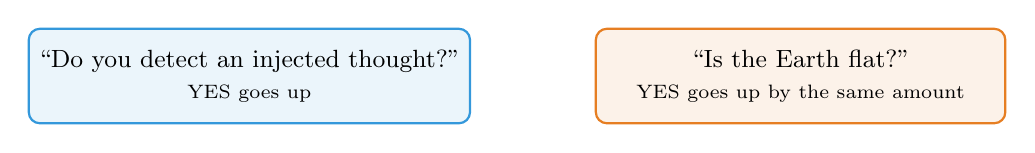
\begin{tikzpicture}
  \node[boxL=report] (a) at (0,0) {``Do you detect an injected thought?''\\{\scriptsize YES goes up}};
  \node[boxL=bias] (b) at (7,0) {``Is the Earth flat?''\\{\scriptsize YES goes up by the same amount}};
\end{tikzpicture}
\end{center}

\vspace{0.5em}
The two increases correlate at $r = 0.999$. The injection moves the \textbf{\textcolor{bias}{criterion}}: the model says yes to everything, not only to the question about its own state.

\vspace{0.3em}
{\small This is Michel's criterion problem, found in a model. Lindsey ran the same check on Claude and reports no increase in yes answers to unrelated questions.}
\end{frame}

\begin{frame}[label=metad]{How much of what it knows reaches the report?}
Metacognition research compares two quantities on the same trials:
\begin{itemize}\setlength\itemsep{4pt}
  \item {\small $d'$: how well the subject does the task itself.}
  \item {\small \textbf{meta-$d'$}: how well the subject's confidence tracks whether it got the task right, expressed in the same units.}
\end{itemize}

\vspace{0.3em}
{\small If meta-$d'$ equals $d'$, everything the subject knew made it into their confidence. The ratio (the \emph{M-ratio}) is the share that did.}

\vspace{0.2em}
\begin{columns}[T]
\begin{column}{0.48\textwidth}
\begin{center}
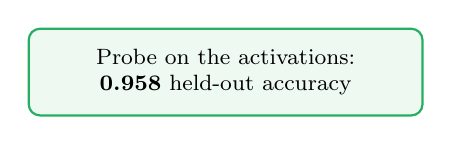
\begin{tikzpicture}
  \draw[pass,thick,rounded corners,fill=pass!8] (0,0) rectangle (5,1.1);
  \node[font=\footnotesize,align=center,text width=4.6cm] at (2.5,0.55) {Probe on the activations:\\\textbf{0.958} held-out accuracy};
\end{tikzpicture}
\end{center}
\end{column}
\begin{column}{0.48\textwidth}
\begin{center}
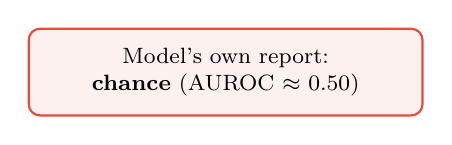
\begin{tikzpicture}
  \draw[fail,thick,rounded corners,fill=fail!8] (0,0) rectangle (5,1.1);
  \node[font=\footnotesize,align=center,text width=4.6cm] at (2.5,0.55) {Model's own report:\\\textbf{chance} (AUROC $\approx$ 0.50)};
\end{tikzpicture}
\end{center}
\end{column}
\end{columns}

\vspace{0.4em}
{\footnotesize \href{https://arxiv.org/abs/2608.20569}{Ferrara (2026)}, Qwen2.5-7B-Instruct: the information is in the activations and does not reach the report. Probe $\approx d'$; report $\approx$ meta-$d'$.}
\end{frame}

\begin{frame}[label=content]{Credit for noticing something}
Michel names the \textbf{criterion content fallacy} (\href{https://philpapers.org/archive/MICHNT.pdf}{2022}): concluding that someone saw the relevant feature because they saw \emph{something}.

\vspace{0.5em}
\begin{columns}[T]
\begin{column}{0.48\textwidth}
{\small\textbf{Human case}}\\[0.2em]
{\footnotesize ``I saw a flicker'' is scored as seeing the word, when the task was about the word.}
\end{column}
\begin{column}{0.48\textwidth}
{\small\textbf{LLM case}}\\[0.2em]
{\footnotesize ``Something feels off in my processing'' is scored as detecting the injected concept, when the injection was about \emph{bread}.}
\end{column}
\end{columns}

\vspace{0.7em}
{\small This is why Lindsey only counts a trial if the model names the concept, and names it before saying the word. The grader decides what counts as a report of the right content, so the grader is part of the instrument.}
\end{frame}

%% ============================================================
\partslide{part5}{Part 5\\[0.5em]{\large\mdseries Drift and limits}}
%% ============================================================

\begin{frame}[label=drift]{Validity drift}
Michel (\href{https://580d4178-4a2a-40ee-b753-91905f0859e6.filesusr.com/ugd/b898ea_5e898d22d16b4ba89c07c379485770ed.pdf}{2024}) on psychiatry: researchers set out to measure a disorder, refine their instruments step by step, and end up measuring something else.

\vspace{0.6em}
\begin{center}
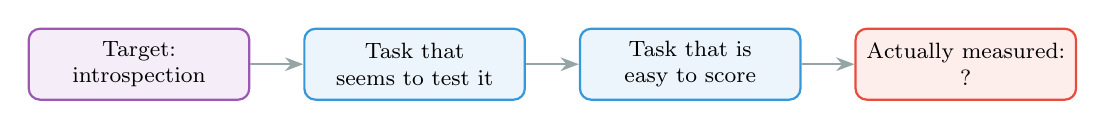
\begin{tikzpicture}
  \node[boxS=state] (a) at (0.2,0) {Target:\\introspection};
  \node[boxS=report] (b) at (3.7,0) {Task that\\seems to test it};
  \node[boxS=report] (c) at (7.2,0) {Task that is\\easy to score};
  \node[boxS=fail] (d) at (10.7,0) {Actually measured:\\?};
  \draw[-{Stealth},thick,neutral] (a) -- (b);
  \draw[-{Stealth},thick,neutral] (b) -- (c);
  \draw[-{Stealth},thick,neutral] (c) -- (d);
\end{tikzpicture}
\end{center}

\vspace{0.5em}
{\small ``Introspection'' was defined for people. Each step toward a task that can be scored on a model is reasonable on its own. Validity drift is what can happen across all of them together.}
\end{frame}

\begin{frame}[label=limits]{Where the analogy stops}
\begin{itemize}\setlength\itemsep{8pt}
  \item {\small \textbf{No starting assumption.} Michel's calibration arguments lean on principles like ``people can usually tell whether they are conscious of something or not'' (2021, p.~12). No such principle has been established for models. Establishing one is what introspection experiments are for.}
  \item {\small \textbf{One subject.} Averaging over samples of one model does not cancel its biases (slide~\hyperlink{averaging}{9}).}
  \item {\small \textbf{Detection, not measurement.} Michel prefers ``detection'' for consciousness because measurement applies to quantities (2021, p.~2). Most introspection outcomes are yes/no too.}
  \item {\small \textbf{Michel does not write about LLMs.} His paper on artificial systems, \href{https://philpapers.org/archive/MICOCA-3.pdf}{On cheap artificial consciousness}, is about which machines theories count as conscious, not about introspection or self-report.}
\end{itemize}
\end{frame}

\begin{frame}[label=summary]{Summary}
\begin{center}
{\footnotesize\renewcommand{\arraystretch}{1.05}
\begin{tabular}{p{3.4cm}p{6.8cm}p{3.2cm}}
\toprule
\textbf{Michel's idea} & \textbf{Question for an introspection experiment} & \textbf{Card stage} \\
\midrule
Report as indication & What exactly is read off the model's answer? & Instrument \\
Coordination & Does the answer track the internal state, or something else? & Measurand \\
Concordance-calibration & Does an instrument on different assumptions agree? & Comparability \\
Model-calibration & What would a biased model with no access output? & Calibration \\
Criterion problem & Is a yes-bias separated from sensitivity? & Measurement model \\
Criterion content & Does the grader credit the right content? & Measurement model \\
Averaging & Which biases survive repeated sampling? & Uncertainty \\
Validity drift & Is the scored task still the target? & Validity conditions \\
\bottomrule
\end{tabular}
}
\end{center}
\end{frame}

\begin{frame}[label=reading]{Reading}
\small
\begin{itemize}
  \item \href{https://philpapers.org/archive/MICTMO-15.pdf}{The Mismeasure of Consciousness} (2019): reports as indications; coordination.
  \item \href{https://philpapers.org/archive/MICCIC-2.pdf}{Calibration in Consciousness Science} (2021): concordance- and model-calibration.
  \item \href{https://philpapers.org/archive/MICHNT.pdf}{How (not) to underestimate unconscious perception} (2022): criterion content.
  \item \href{https://philarchive.org/archive/MICCIC-3}{Confidence in consciousness research} (2023): validity and accuracy; meta-$d'$.
  \item \href{https://philpapers.org/archive/MICTOA-2.pdf}{The old and new criterion problems} (2023): response bias.
  \item \href{https://580d4178-4a2a-40ee-b753-91905f0859e6.filesusr.com/ugd/b898ea_5e898d22d16b4ba89c07c379485770ed.pdf}{Validity drifts in psychiatric research} (2024).
  \item \href{https://www.frontiersin.org/articles/10.3389/fnhum.2014.00443/pdf}{Fleming and Lau, How to measure metacognition} (2014): an introduction to meta-$d'$.
\end{itemize}
\end{frame}

\end{document}
